\chapter{Control Unit}
The Control Unit is the component that directs the operations of the processor. \\
There are different possibilities for its implementation and we choose the hardwired one: \\
the control hardware it is a finite state machine that switches from a state to another at every clock cycle, generating a sequence of individual bits represent various control signals (i.e. the control word). \\
\\
\begin{figure}[h!]
	\centering
	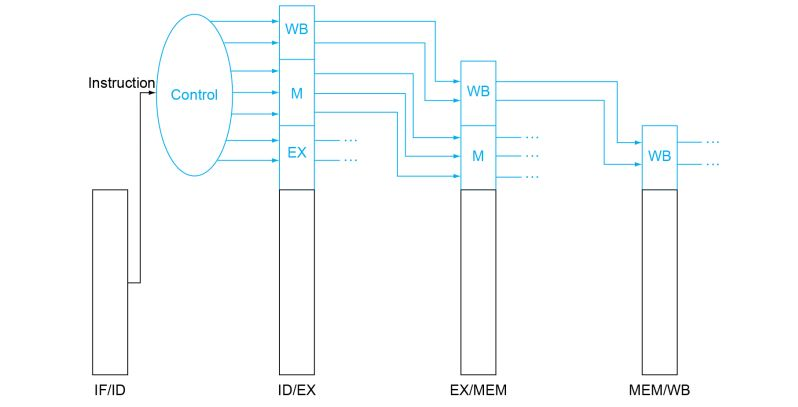
\includegraphics[width=12cm]{./images/structure_CU}
	\caption{General CU structure}
	\label{fig3.1}
\end{figure}

\section{Control Word Generation}
The component receives as input the instruction and based on the instruction's Opcode, it decides which CW it has to send to the output. \\
This selection is based on the bits in position 2, 4, 5, 6. \\
\\
This because we have found that these are the bits which, once concatenated together, identify each instruction uniquely.\\
These bits are used to access to the matrix which generates the corrispondent CW.\\
\begin{figure}[h!]
	\centering
	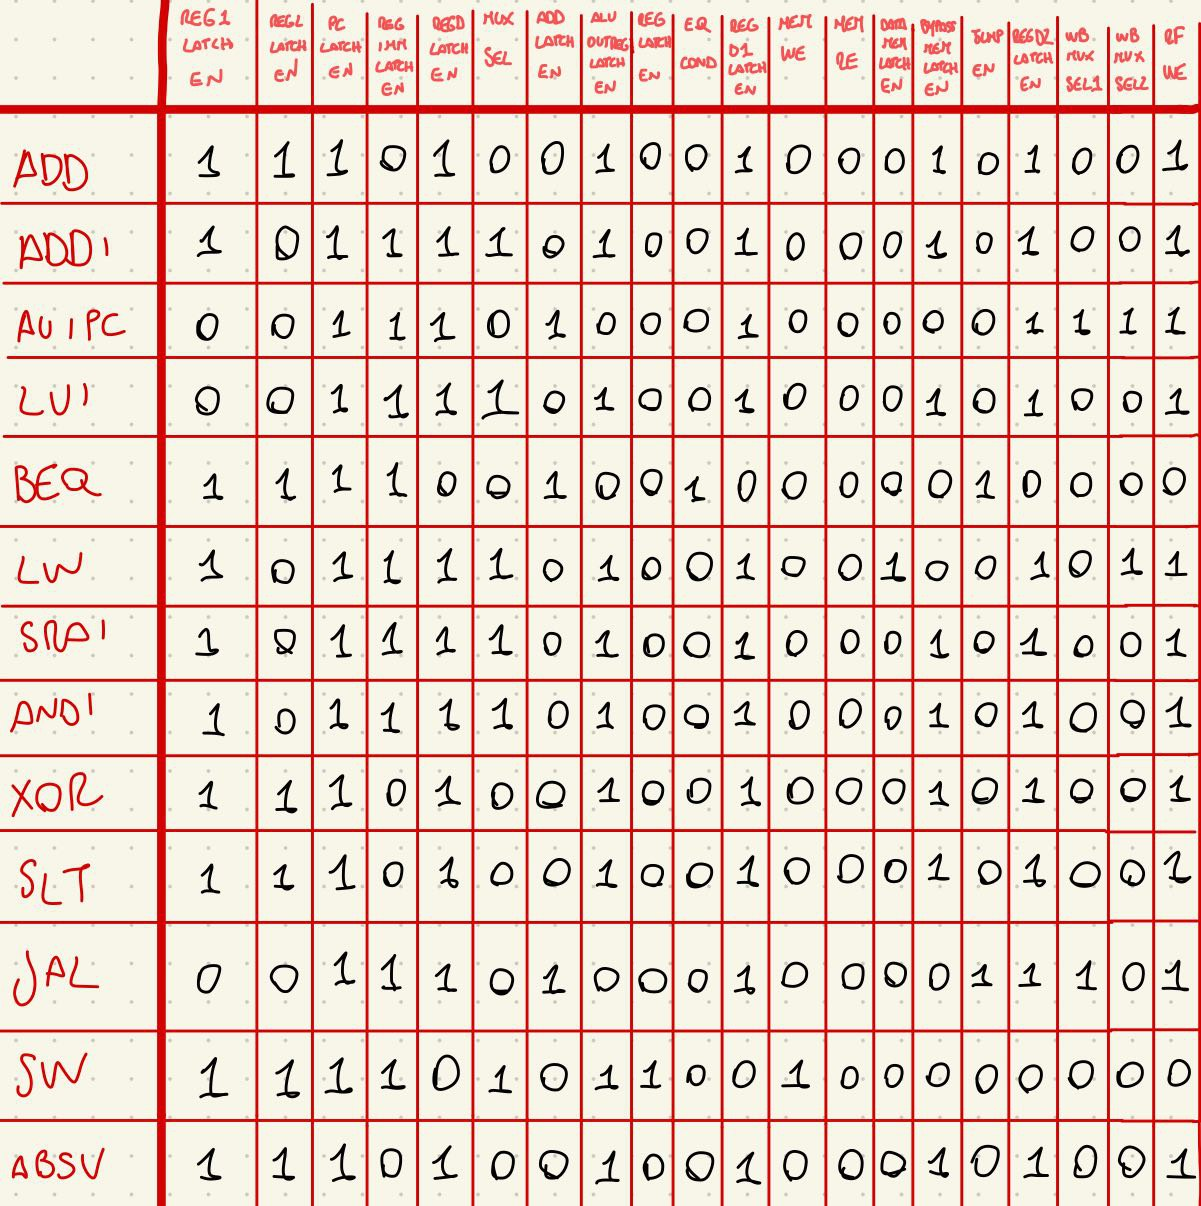
\includegraphics[width=16cm]{./images/control_signals}
	\caption{Control signal of each instruction}
	\label{fig3.3}
\end{figure}
Each instruction has its own control signals, but they are the same for instructions belonging to the same class (exept for some that belong to a class, but they have different control signals):\\
\\
\begin{itemize}
	\item I-type (ADDI, SRAI, ANDI);
	\item LW (I-type);
	\item R-type (ADD, XOR, SLT);
	\item B-type (BEQ);
	\item J-type (JAL);
	\item S-type (SW);
	\item AUIPC (U-type);
	\item LUI (U-type);		
\end{itemize}
\section{ALU Opcode generation}
The second process present in the CU is the one dedicated to the generation of the code destinated to the ALU, in order to determine its behavior.
Its sensitivity list comprehend the instruction's OPCODE and the instruction's FUNCT and it follows the following scheme:\\
\\
\begin{itemize}
	\item I-type -$>$ OPCODE = "0010011" :
		\begin{itemize}
			\item ADDI -$>$ FUNCT = "000";
			\item SRAI -$>$ FUNCT = "101";
			\item ANDI -$>$ FUNCT = "111";
		\end{itemize}
	\item LW (I-type) -$>$ OPCODE = "0000011";
	\item R-type -> OPCODE = "0110011":
		\begin{itemize}
			\item ADD -$>$ FUNCT = "000";
			\item XOR -$>$ FUNCT = "100";
			\item SLT -$>$ FUNCT = "010";
		\end{itemize}
	\item B-type (BEQ) -$>$ OPCODE = "1100011";
	\item J-type (JAL) -$>$ OPCODE = "1101111";
	\item S-type (SW) -$>$ OPCODE = "0100011";
	\item AUIPC (U-type) -$>$ OPCODE = "0010111";
	\item LUI (U-type) -$>$ OPCODE = "0110111";		
\end{itemize}